
\section{Experiments}
\paragraph{Implementation Details.}
We adopt Wan-2.1-1.3B~\cite{wan2025} as our base model. It contains 1.3B parameters, and our GA introduces additional 0.6B parameters. Our proposed data curation pipeline produced 75K+ paired video samples from the training splits of DL3DV~\cite{ling2024dl3dv} and RE10K~\cite{re10k}, each with 81 frames.  We hold out their test splits for evaluation. We use Gemini-Flash-2.5~\cite{gemini2.5flash} to generate the text description of each video. We train our model on 8 H200 GPUs for 100K steps with a batch size of 8 and a frame resolution of 480$\times$832. Training uses the AdamW optimizer with a linear learning rate (LR) warm-up over the first 1K steps, followed by a constant LR of 1$\times$10$^{-5}$. We randomly drop out geometry modalities and text input during training. 


\paragraph{Experimental Setup.} We evaluate our method on common novel-view synthesis benchmarks: DL3DV~\cite{ling2024dl3dv} and RE10K~\cite{re10k}.
Testing scenes are drawn from the official test splits of each dataset, which remain unseen during training. 
For DL3DV and RE10K, we randomly downsample 5\% of the original video frames as training views and optimize Gaussian splats for 7K iterations following the standard Splatfacto~\cite{ye2025gsplat} setup. The remaining views are held out for evaluation. All methods are tested at their native operating resolution and resized to 480$\times$832 for comparison.



\paragraph{Baselines and Metrics.}
We compare our method against open-source, state-of-the-art approaches, including  DiFiX3D+~\cite{wu2025difix3d},  GenFusion~\cite{Wu2025GenFusion}, and ExploreGS~\cite{Kim_2025_ExploreGS}. We also compare against MVSplat360~\cite{chen2024mvsplat360} on feed-forward view synthesis, a model coupled with MVSplat~\cite{chen2024mvsplat}. Each baseline employs slightly different camera sampling strategies and reconstruction heuristics, making it difficult to disentangle improvements due to model design from those due to optimization choices. 
To ensure a fair comparison, we run all baselines on the same renderings and apply the same reconstruction update strategy described in \cref{subsec:refining_3d}. 
All baselines are evaluated using their official implementations and publicly released weights. 
We assess performance using standard image and perceptual quality metrics: PSNR, SSIM~\cite{ssim}, LPIPS~\cite{lpips}, and FID~\cite{NIPS2017_8a1d6947}. In the following, best results are highlighted as\colorbox{colorFst}{\bf first},\colorbox{colorSnd}{second}, and\colorbox{colorTrd}{third}.





\begin{table}[t]
\centering
\footnotesize
\setlength{\tabcolsep}{4pt}
\begin{tabular}{lcccc}
\toprule
\textbf{Feed-forward Method} & \textbf{PSNR $\uparrow$} & \textbf{SSIM $\uparrow$} & \textbf{LPIPS $\downarrow$} & \textbf{FID $\downarrow$}\\
\midrule
DepthSplat~\cite{xu2024depthsplat} & \nd21.773 & \nd0.842 & \nd0.278  &\rd28.903\\
\quad \textit{w/ }Difix3D+~\cite{wu2025difix3d} & \rd21.415 & \rd0.837 & \rd0.303 & \nd17.968 \\
\quad \textit{w/ }ExploreGS~\cite{Kim_2025_ExploreGS} & 21.195 & 0.816 & 0.317 & 35.475\\
\quad \textit{w/ }\ours(Ours) & \fs 22.802 & \fs 0.848 & \fs0.258 & \fs15.128 \\
\midrule
MVSplat~\cite{chen2024mvsplat} & \rd18.744 & \rd0.706 & \rd0.375 & 44.479\\
% \quad \textit{w/ }MVSplat360~\cite{chen2024mvsplat360} & & & & \\
\quad \textit{w/ }Difix3D+~\cite{wu2025difix3d} & 18.261 & 0.702 & 0.385 & \nd23.954\\
\quad \textit{w/ }ExploreGS~\cite{Kim_2025_ExploreGS} & 18.112 & 0.692 & 0.389 & \rd36.390\\
\quad \textit{w/ }MVSplat360~\cite{chen2024mvsplat360} & \fs19.819&\fs0.747 & \nd0.354& 36.821\\
\quad \textit{w/ }\ours(Ours)  & \nd19.756 & \nd0.744 & \fs0.338 & 
\fs23.823\\
\bottomrule
\end{tabular}
\caption{\textbf{Feed-forward View Synthesis Results on RE10K~\cite{re10k}.} Our method consistently improves feed-forward 3DGS reconstruction on different backbones while baseline methods Difix3D and ExploreGS decrease the consistency with the original scene. MVSplat360 is on par to our method in terms of consistency within its specialized domain, but still lacks in visual quality.}
\label{tab:feedforward_refine}
\end{table}
 
\begin{table}[t]
\centering
\footnotesize
    \centering
    \setlength{\tabcolsep}{1pt}
    \begin{tabular}{lcccccc}
    \toprule
     & \multicolumn{3}{c}{\textbf{DL3DV}} 
     & \multicolumn{3}{c}{\textbf{RE10K}} \\
     \midrule
     \textbf{Method} 
     & PSNR $\uparrow$ & SSIM $\uparrow$ & LPIPS $\downarrow$ 
     & PSNR $\uparrow$ & SSIM $\uparrow$ & LPIPS $\downarrow$ \\
    \midrule
    Splatfacto~\cite{ye2025gsplat} & 17.42 & 0.605 &	0.412 &	19.23 & 0.708 &	0.457 \\
    GenFusion~\cite{Wu2025GenFusion} & 18.08 &	\rd0.615 &	 0.421&	19.52 &	0.719 & 0.329 \\
    Difix3D+~\cite{wu2025difix3d} & \nd18.87 & \nd0.626 &	\fs0.265 & \rd 21.98	 &	\nd0.767 &	\nd0.187 \\
    ExploreGS~\cite{Kim_2025_ExploreGS} &\rd18.71 & 0.611& \rd0.377&\nd22.06 & \rd0.742 & \rd0.257\\
    \ours (Ours) & \fs19.36 &	\fs0.628 &	\nd0.279 &	\fs24.17 & \fs0.817 & \fs0.175 \\
    
    \bottomrule
    \end{tabular}
    \caption{\textbf{Performance on Improving 3D Reconstruction}. \ours demonstrates superior performance on most metrics, showcasing the multi-view consistency in our enhanced frames. }
    \label{tab:splat_refine}
\end{table}

\begin{figure*}[t]
    \centering
 \begin{tabular}{cccccc}
   
    \multicolumn{6}{c}{%
        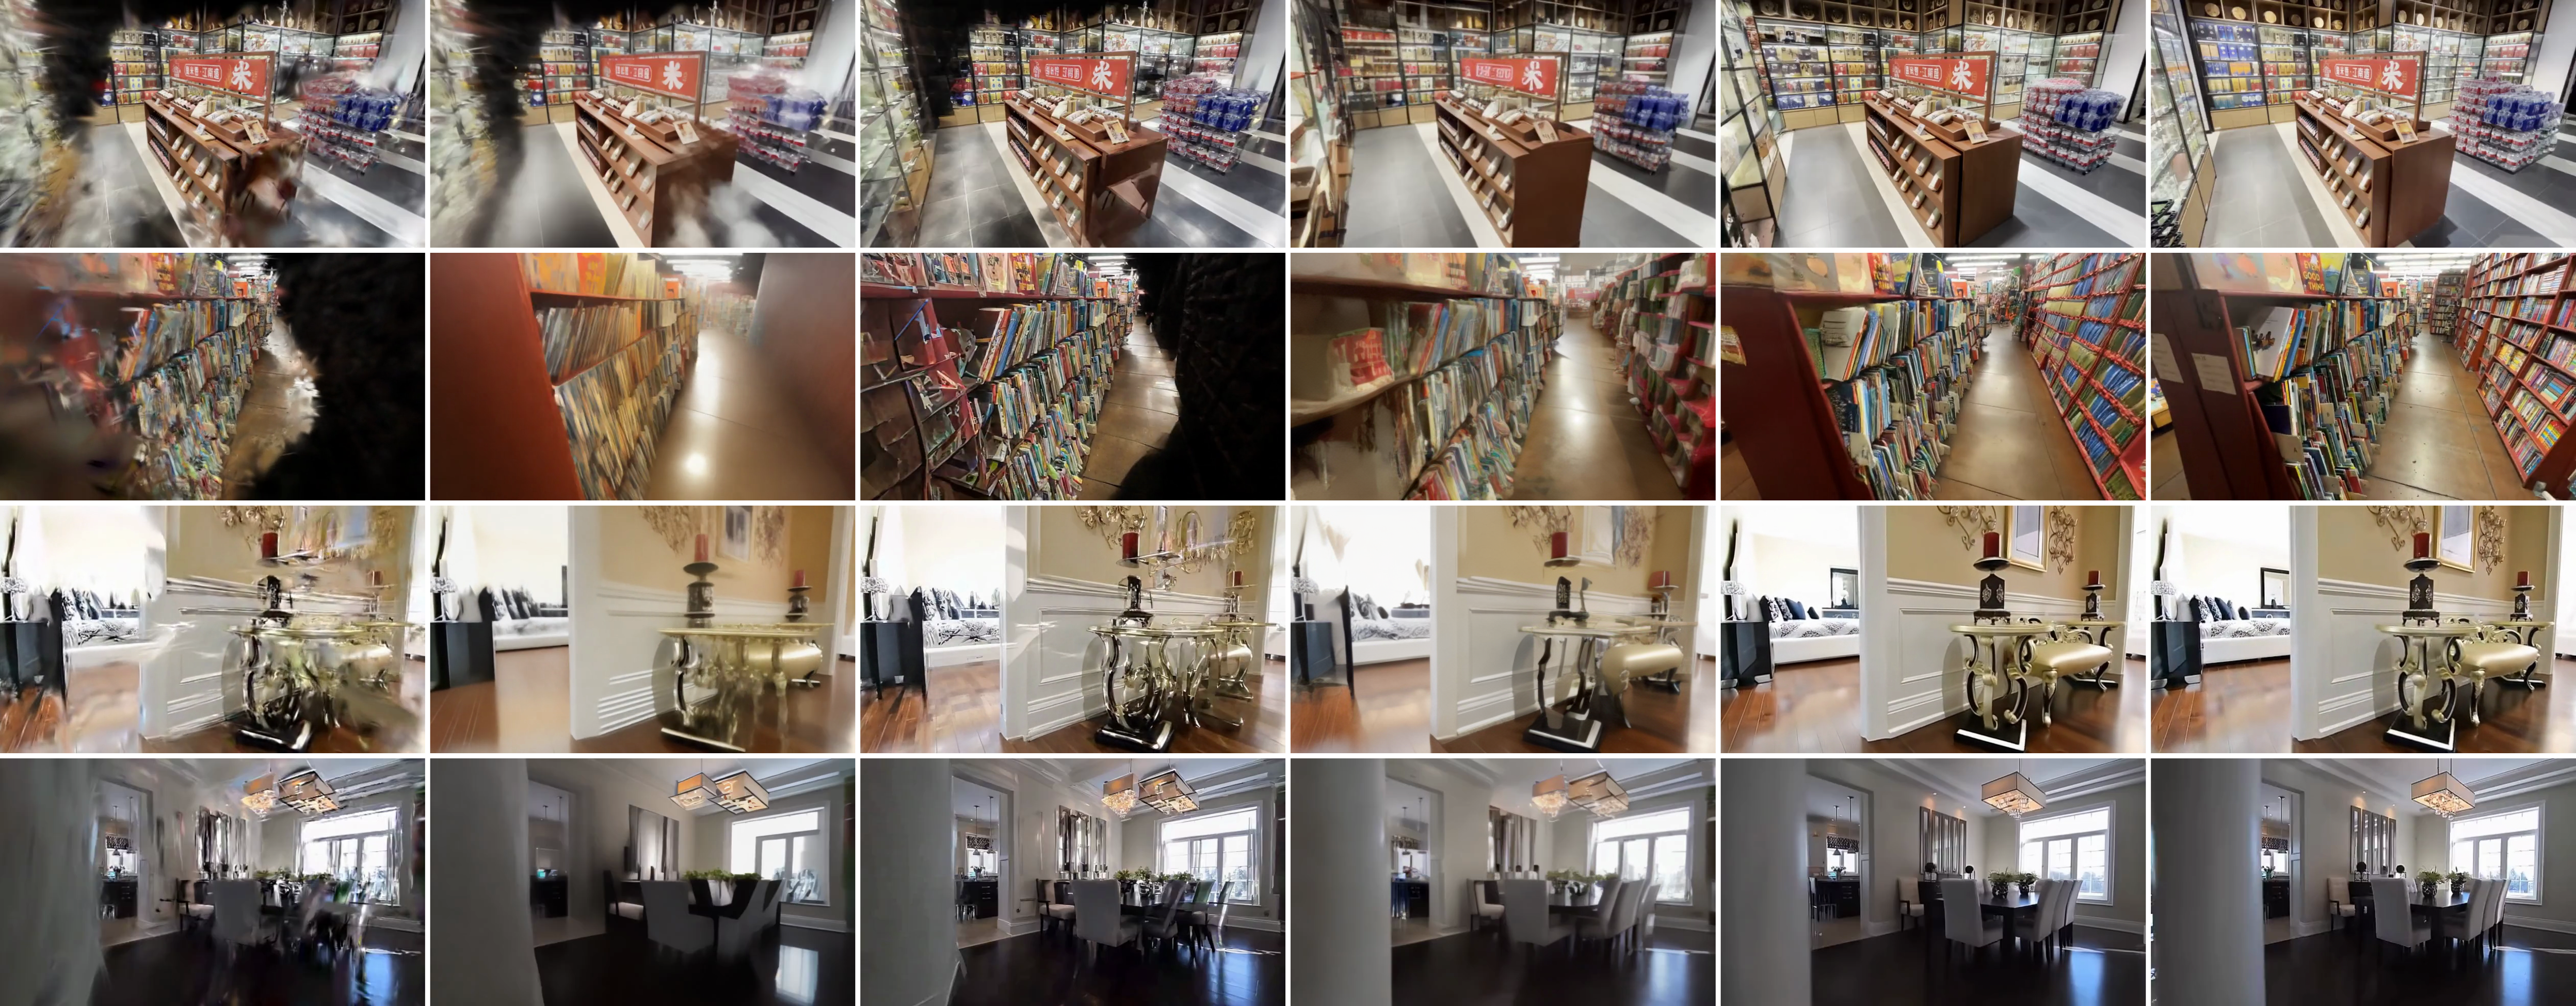
\includegraphics[width=\linewidth]{fig/image/main_comparison.png}%
    } \\
     \hspace{0.4cm} \small Splatfacto~\cite{ye2025gsplat} & 
    \hspace{0.4cm} \small GenFusion~\cite{Wu2025GenFusion} & 
    \hspace{.5cm}\small Difix3D+~\cite{wu2025difix3d} & 
    \hspace{.6cm}\small ExploreGS~\cite{Kim_2025_ExploreGS} &
    \hspace{0.2cm}\small \ours (Ours) & 
    \hspace{-0.1cm}\small Ground Truth \\
    \midrule
    \multicolumn{6}{c}{%
        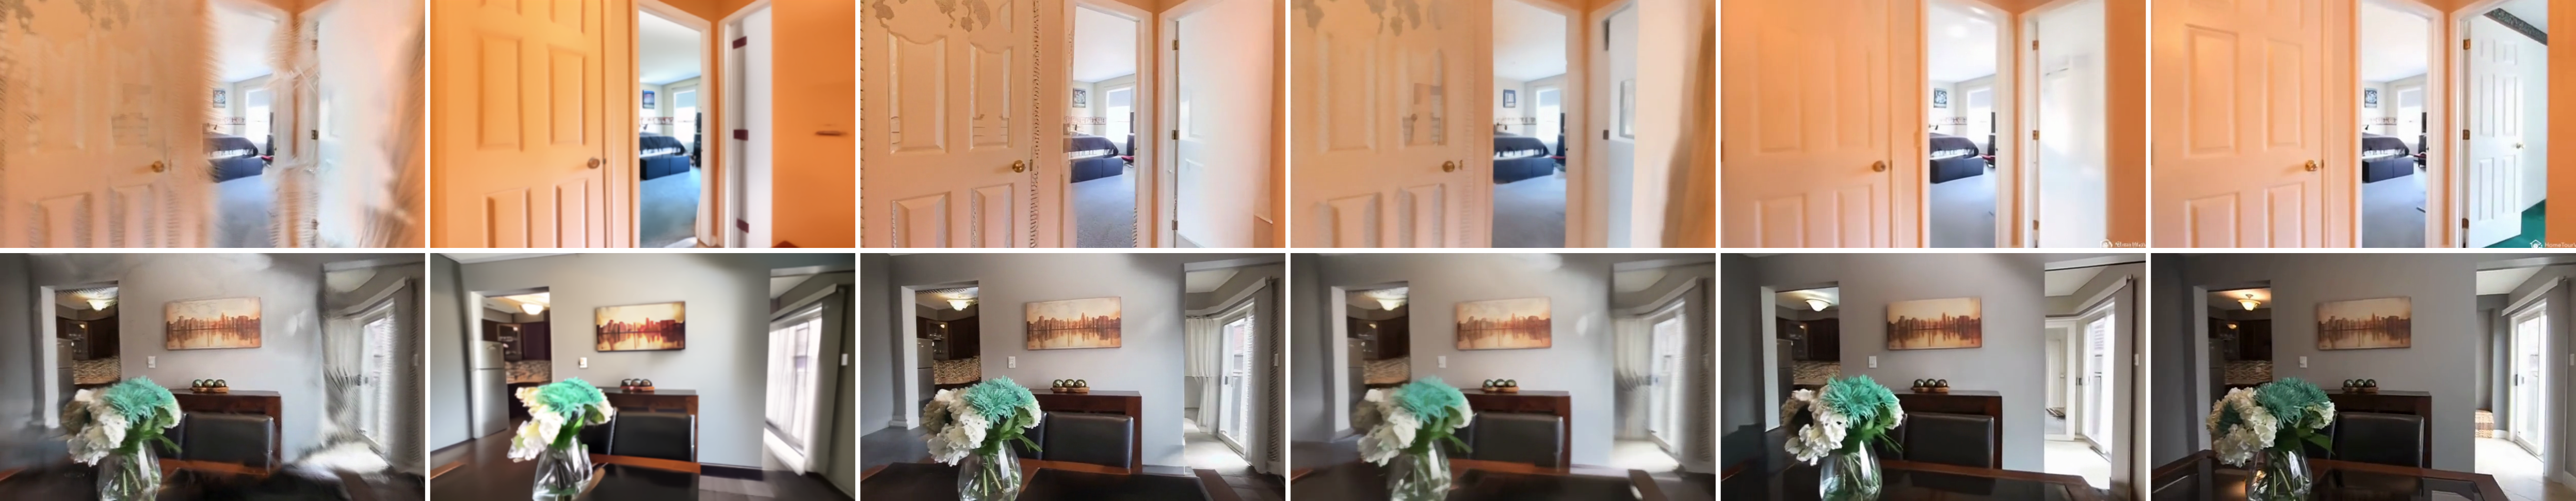
\includegraphics[width=\linewidth]{fig/image/main_comparison_part2.png}%
    } \\
    \hspace{0.4cm} \small DepthSplat~\cite{xu2024depthsplat} & 
    \hspace{0.4cm} \small MVSplat360~\cite{chen2024mvsplat360} & 
    \hspace{.5cm}\small Difix3D+~\cite{wu2025difix3d} & 
    \hspace{.6cm}\small ExploreGS~\cite{Kim_2025_ExploreGS} &
    \hspace{0.2cm}\small \ours (Ours) & 
    \hspace{-0.1cm}\small Ground Truth \\

\end{tabular}  
   \caption{\textbf{Qualitative Comparison on Novel-View Refinement.}
We compare \ours with baseline methods on diverse scenes from DL3DV~\cite{ling2024dl3dv} and RE10K~\cite{re10k}. 
\ours effectively removes rendering artifacts such as blur, floaters, ghosting, and texture distortions, producing sharper geometry, cleaner reconstruction than Splatfacto~\cite{ye2025gsplat}, GenFusion~\cite{Wu2025GenFusion}, DiFiX3D+~\cite{wu2025difix3d}, and ExploreGS~\cite{Kim_2025_ExploreGS}, and achieving visual fidelity closest to the ground truth. 
From top to bottom, our model demonstrates strong generalization across various refinement scenarios: (\textit{1}) inpainting missing regions, (\textit{2}) outpainting beyond the original view, (\textit{3–4}) correcting blur, ghosting, and geometric errors, and (\textit{5–6}) handling artifacts from feed-forward 3DGS models, including transparent Gaussian primitives and spiky geometry. 
% While baselines handle certain artifact types, they fail to generalize as robustly as \ours.
}

    \label{fig:image_refine}
\end{figure*}


% \begin{figure*}[t]
%     \centering
%     \setlength{\tabcolsep}{3pt} % tighten columns a bit
%     \renewcommand{\arraystretch}{1.0}
%     \begin{tabular}{@{}p{1.6cm}cccccc@{}} % <-- left label column
%         % -------- TOP BLOCK (4 rows inside the image) --------
%         \multirow{1}{*}{\centering
%             \rotatebox{90}{\parbox{3.2cm}{\centering \small Optimization-based\\[-2pt] 3DGS}}
%         }
%         & \multicolumn{6}{c}{%
%             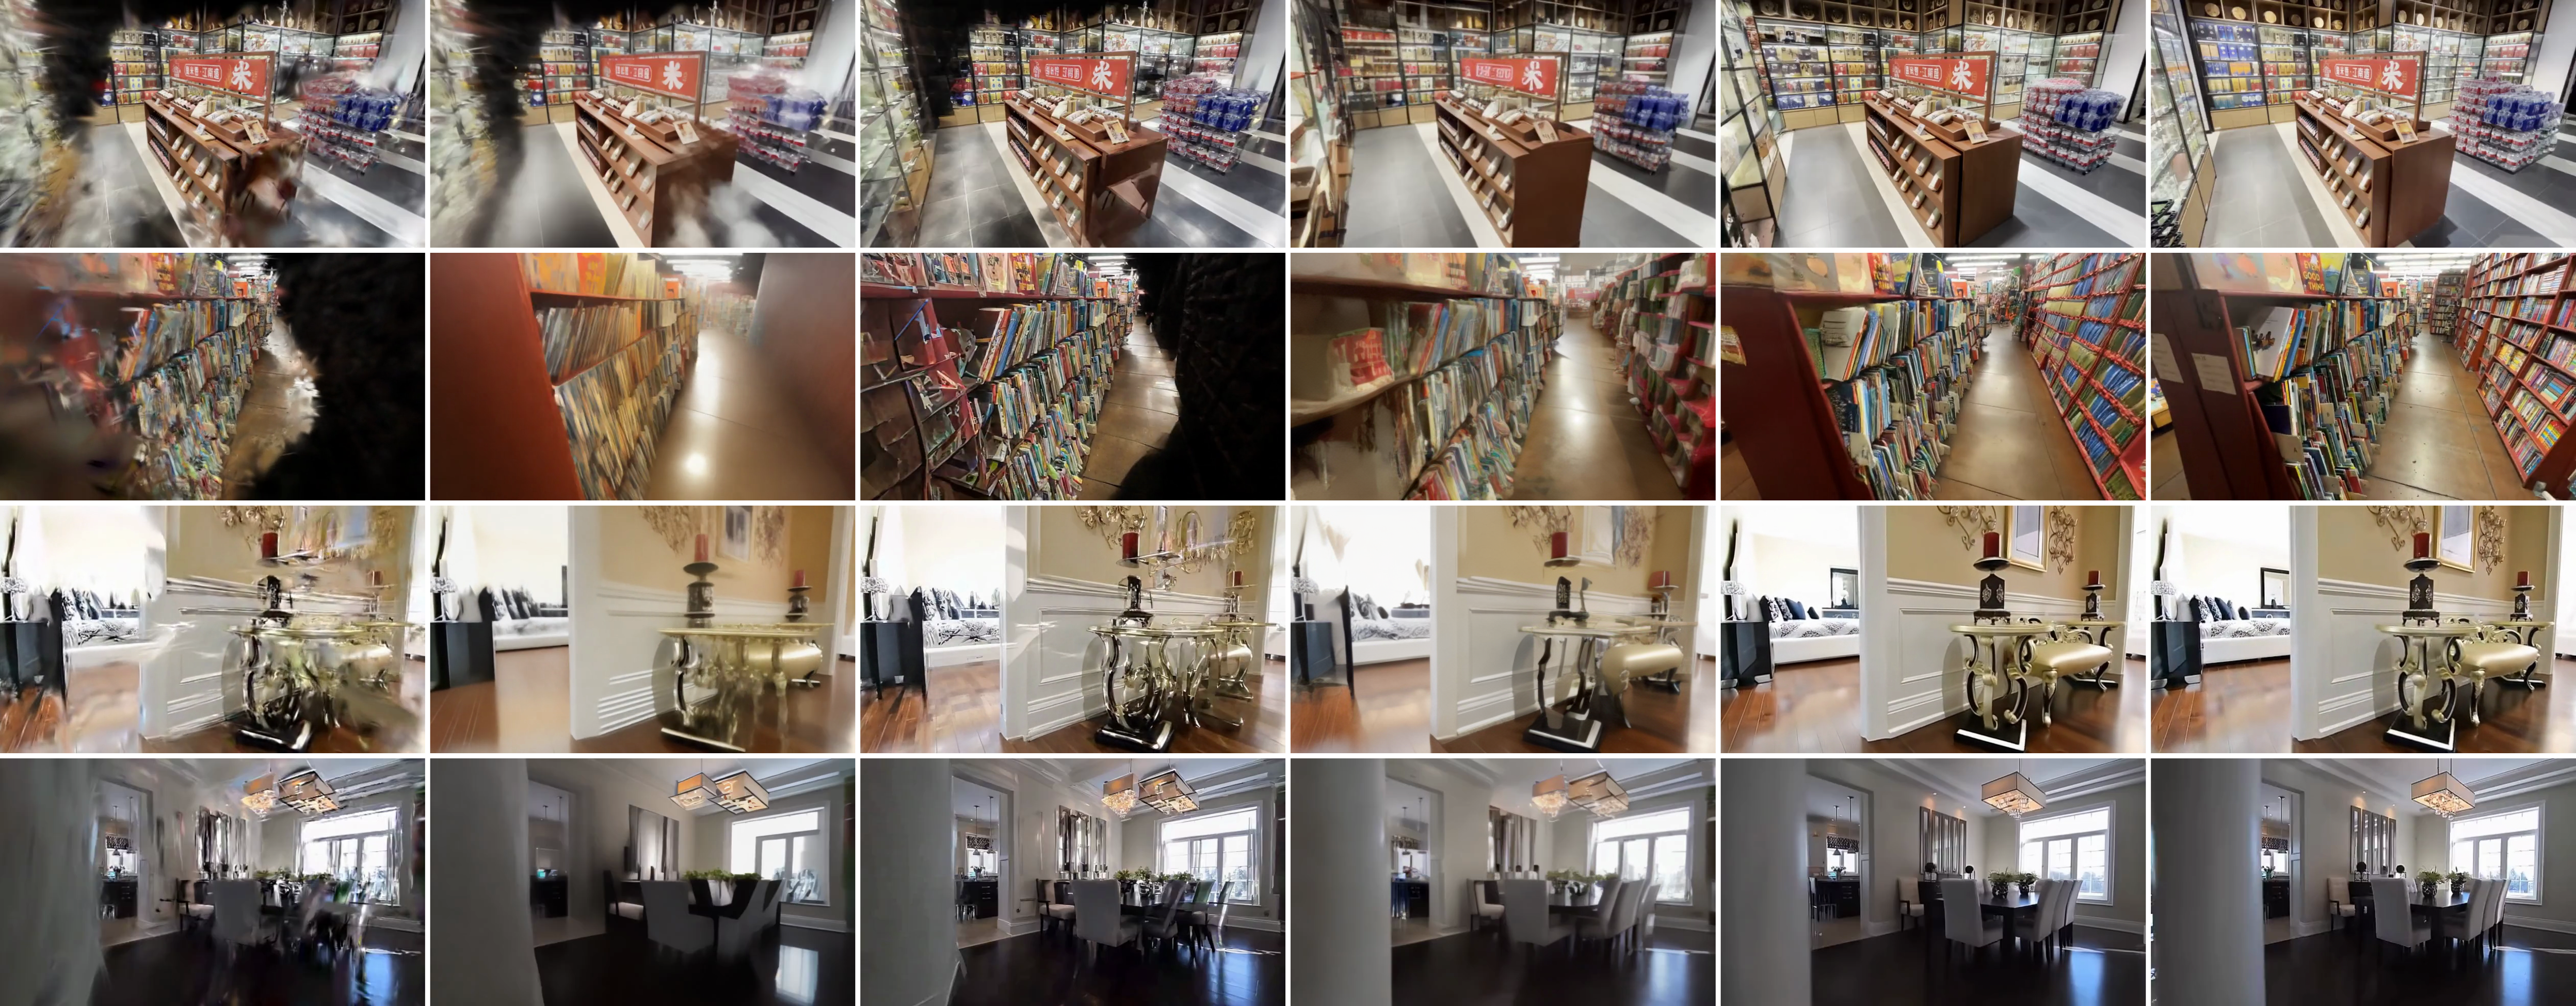
\includegraphics[width=\linewidth]{fig/image/main_comparison.png}%
%         } \\
%         & \hspace{0.4cm} \small Splafacto~\cite{ye2025gsplat} &
%           \hspace{0.4cm} \small GenFusion~\cite{Wu2025GenFusion} &
%           \hspace{.5cm}\small Difix3D+~\cite{wu2025difix3d} &
%           \hspace{.6cm}\small ExploreGS~\cite{Kim_2025_ExploreGS} &
%           \hspace{0.2cm}\small \ours (Ours) &
%           \hspace{-0.1cm}\small Ground Truth \\
%         \midrule
%         % -------- BOTTOM BLOCK (2 rows inside the image) --------
%         \multirow{2}{*}{\centering
%             \rotatebox{90}{\parbox{3.2cm}{\centering \small Feed-forward\\[-2pt] 3DGS}}
%         }
%         & \multicolumn{6}{c}{%
%             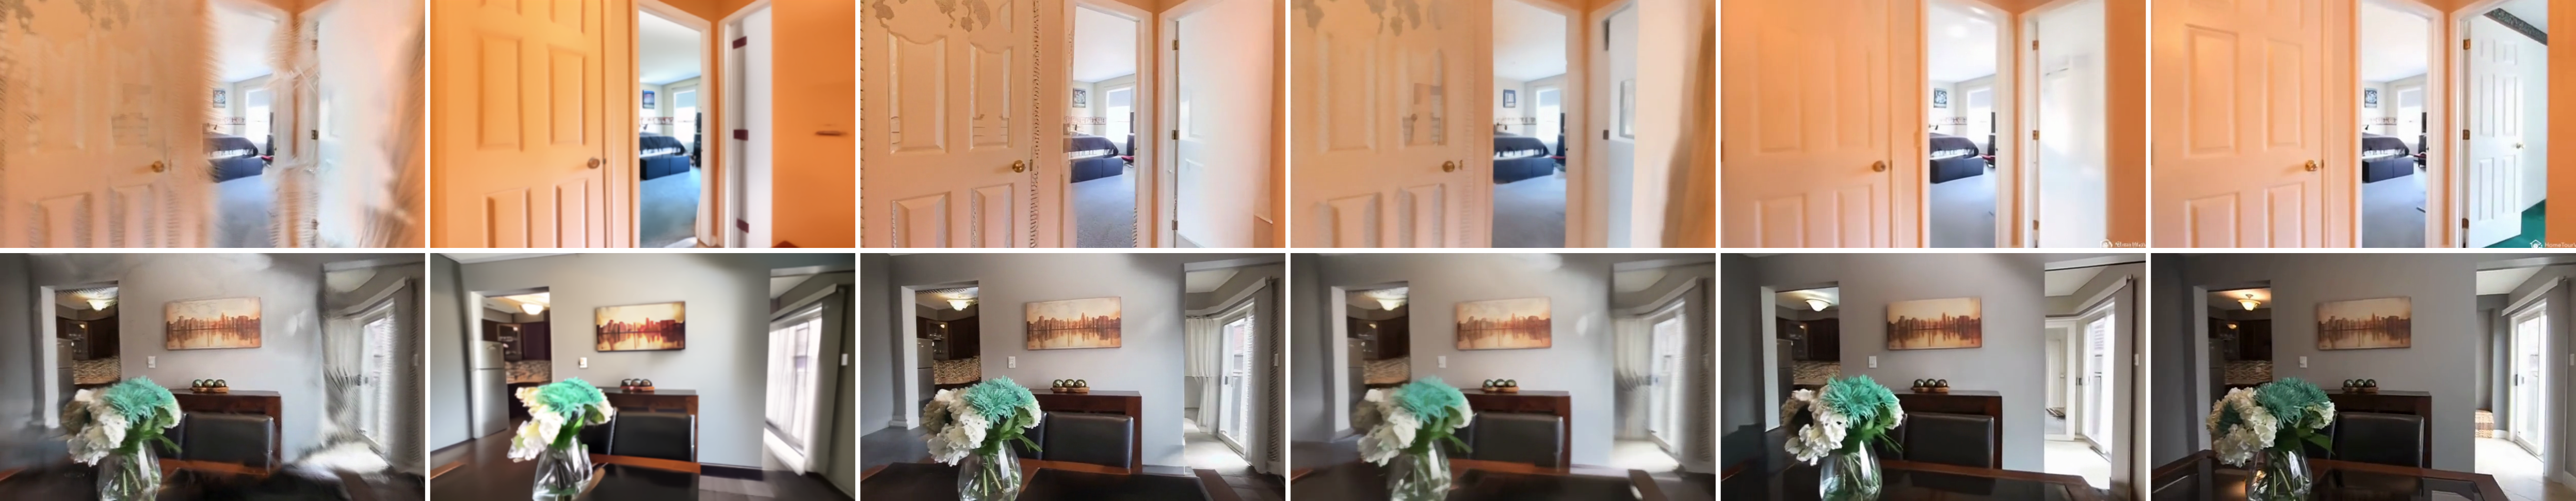
\includegraphics[width=\linewidth]{fig/image/main_comparison_part2.png}%
%         } \\
%         & \hspace{0.4cm} \small DepthSplat~\cite{xu2024depthsplat} &
%           \hspace{0.4cm} \small GenFusion~\cite{Wu2025GenFusion} &
%           \hspace{.5cm}\small Difix3D+~\cite{wu2025difix3d} &
%           \hspace{.6cm}\small ExploreGS~\cite{Kim_2025_ExploreGS} &
%           \hspace{0.2cm}\small \ours (Ours) &
%           \hspace{-0.1cm}\small Ground Truth \\
%     \end{tabular}
%     \caption{\textbf{Qualitative Comparison on Novel-View Refinement.} ...}
%     \label{fig:image_refine}
% \end{figure*}




\subsection{Results}
\paragraph{Improving Novel-View Synthesis.}
We first evaluate performance on pure rendering refinement, \ie, novel-view synthesis, as reported in Table~\ref{tab:recon_perf}. We compare three variants of our model: \textit{Ours (Single)}, trained solely on DL3DV~\cite{ling2024dl3dv} with optimization-based data; \textit{Ours (Joint)}, jointly trained on all datasets with the complete artifact data; and \textit{Ours (Distilled)}, our distilled 4-step model. The model trained exclusively on DL3DV outperforms all baselines trained on the same dataset by a substantial margin in terms of image quality.

Difix3D+~\cite{wu2025difix3d}, based on an image diffusion model, processes frames independently and thus lacks multi-view consistency and performs poorly on removing floaters. GenFusion~\cite{Wu2025GenFusion} and ExploreGS~\cite{Kim_2025_ExploreGS}, though leveraging a video diffusion framework, achieve lower performance due to insufficient conditioning signals compared to our GP-buffer and sub-optimal conditioning strategy, which impairs temporal coherence. More importantly, we find our joint trained model has improved performance compared to training on a single dataset, indicating that exposure to diverse reconstruction artifacts and scene types enhances the model’s performance on the same dataset, demonstrating the importance of mix training across different datasets and methods.
\cref{fig:image_refine} further confirms our method's superior performance: the four different examples examine the model's ability in inpainting, outpainting, sharpening the blurry, and correcting wrong geometry in the original rendering.

\paragraph{Improving Feed-Forward View Synthesis.}
We evaluate our model’s ability to refine renderings produced by feed-forward 3DGS reconstruction methods, DepthSplat~\cite{xu2024depthsplat} and MVSplat~\cite{chen2024mvsplat}, as reported in \cref{tab:feedforward_refine}. Prior refinement approaches generally struggle on feed-forward reconstructions—MVSplat360~\cite{chen2024mvsplat360} being the sole exception, as it is explicitly tailored for MVSplat. In contrast, \ours generalizes effectively across different feed-forward backbones.
Although our method is evaluated on MVSplat outputs without ever being trained on MVSplat predictions, it performs on par with MVSplat360, which is fully trained on that setting. Qualitative results in \cref{fig:image_refine} further confirm that our method can reliably correct spiky primitives and semi-transparent Gaussian artifacts.


\vspace{-10pt}

\paragraph{Inference Speed.}
We report inference speed in \cref{tab:recon_perf}, measuring the average frame rate based on end-to-end inference time on a single H200 GPU. Our distilled model maintains comparable PSNR, SSIM, and LPIPS to the non-distilled version, while surpassing all baselines with a real-time speed of 16~FPS. A slightly higher FID score is observed, which we attribute to the reduced number of denoising steps and minor loss of high-frequency details.


\begin{figure}[t]
    % \centering
    \includegraphics[width=\linewidth]{fig/image/recon_v3.pdf}%
   \caption{\textbf{Qualitative Comparison on 3D Reconstruction.} We show the novel-view renderings from the improved 3D reconstruction refined using enhanced views from different methods.
   \ours consistently outperforms baseline methods. }
    \label{fig:recon_comparison}
\end{figure}



\paragraph{Improving 3D Reconstruction.}
We evaluate the effectiveness of \ours in enhancing the underlying 3DGS representation rather than only refining individual frames. 
This task jointly measures rendering fidelity and 3D consistency, with metrics reported per scene to assess holistic reconstruction quality. 
As shown in \cref{tab:splat_refine}, \ours achieves superior PSNR and SSIM across datasets, with occasionally slightly higher LPIPS than Difix3D due to its perceptual loss during training. 
Overall, \ours produces sharper, cleaner, and more consistent reconstructions, significantly improving both rendering quality and geometric coherence (see \cref{fig:recon_comparison}).








\subsection{Ablation Studies}
We validate our key design choices from three perspectives: input modalities, training data, and model architecture.
\vspace{-5mm}

\begin{table}[t]
\centering
\scriptsize
\setlength{\tabcolsep}{3pt}
\begin{tabular}{ccccc|ccccc}
\toprule
\multicolumn{5}{c}{\textbf{Input Modality}} & \multicolumn{4}{c}{\textbf{Performance}} \\
RGB & Depth & Normal & Alpha & Cov. & PSNR$\uparrow$ & SSIM$\uparrow$ & LPIPS$\downarrow$ & FID$\downarrow$ \\
\midrule
\checkmark &  &  &  &  & 19.148 & 0.719 & 0.385 & 15.451 \\
\checkmark & \checkmark &  &  &  & 19.289 & 0.726 & 0.361 & 10.542 \\
\checkmark & \checkmark & \checkmark &  &  & 19.744 & 0.738 & 0.355 & 10.291 \\
\checkmark & \checkmark & \checkmark & \checkmark &  & 19.958 & 0.748 & 0.344 & 8.612 \\
\checkmark & \checkmark & \checkmark & \checkmark & \checkmark & \fs20.753 & \fs0.773 & \fs0.329 & \fs6.724 \\
\bottomrule
\end{tabular}
\caption{\textbf{Ablation on Input Modalities on DL3DV Dataset.} Inclusion of more geometric cues (depth, normal, alpha, covariance) improves reconstruction fidelity and perceptual quality. 
}
\label{tab:ablation_modalities}
\end{table}

\paragraph{Input Modality.} We analyze the contribution of each geometric channel in the GP-Buffer by training five separate models, each with a different combination of input modalities. For efficiency, all models are trained on one-third of the full dataset. As per \cref{tab:ablation_modalities}, adding geometric modalities (depth, normal, alpha, covariance) leads to consistent improvements in rendering accuracy and perceptual quality. \cref{fig:gbuffer} further confirms that GP-buffer can better disambiguate noisy regions and produce sharper reconstructions.

\begin{figure}[t]
    \centering
    \includegraphics[width=.7\linewidth]{fig/image/ablation_gbuffer.pdf}
    \caption{\textbf{Qualitative Ablation on GP-Buffer.} Additional geometric attributes help the model “see through” floaters and blur, producing cleaner and sharper results than RGB-only.}
    \label{fig:gbuffer}
\end{figure}



\paragraph{Artifact Simulation (Data).}
To isolate data generation from architecture, we fix the backbone and training setup, and compare prior artifact synthesis~\cite{Kim_2025_ExploreGS,Wu2025GenFusion,wu2025difix3d} only using uniform view downsampling and splat underfitting, against our proposed pipeline (Sec.~\ref{sec:data}), which combines optimization- and feed-forward degradations while injecting pose and coverage diversity. 
Our synthesis yields higher PSNR/SSIM and lower LPIPS/FID (Tab.~\ref{tab:ablation_artifact}, rows 1\&3). Training with a \emph{mixed} artifact set improves both feed-forward \emph{and} optimization-based evaluations (Tab.~\ref{tab:splat_refine}), suggesting that exposure to cross-paradigm artifacts produces a more balanced refiner rather than overfitting to one pipeline.


\begin{table}[t]
\centering
\scriptsize
\setlength{\tabcolsep}{5pt}
\begin{tabular}{lc|cccc}
\toprule
\multicolumn{2}{c|}{\textbf{Training Config.}} & \multicolumn{4}{c}{\textbf{Performance}} \\
Artifact Sim. & Architecture & PSNR$\uparrow$ & SSIM$\uparrow$ & LPIPS$\downarrow$ & FID$\downarrow$ \\
\midrule
Baseline & \textit{w/.} GA & \nd21.087 & \rd0.789 & \nd0.303 & \rd5.717 \\
Ours & \textit{w/o.} GA & \rd20.904 & \nd0.794 & \rd0.308 & \nd5.296 \\
Ours & \textit{w/.} GA & \fs22.548 & \fs0.832 & \fs0.278 & \fs3.933 \\
\bottomrule
\end{tabular}
\caption{\textbf{Ablation on Artifact Simulation and Architecture.} Evaluating the impact of artifact simulation and geometry adapter block on reconstruction fidelity and perceptual quality.}
\label{tab:ablation_artifact}
\end{table}


\paragraph{Geometry Adapter.} 
Existing methods such as GenFusion~\cite{Wu2025GenFusion} and ExploreGS~\cite{Kim_2025_ExploreGS} condition generation by directly adding conditioning latents to the noised latents. 
We find this strategy suboptimal: as shown in \cref{tab:ablation_artifact} (rows 2\&3), replacing our GA with a simple convolutional fusion layer (\textit{w/o GA}) yields slower convergence and weaker geometric alignment between conditioning and target structures. 
In contrast, incorporating our GA consistently improves all metrics, raising PSNR from 20.90 to 22.55 and reducing LPIPS and FID by 0.03 and 1.36, respectively. 